\documentclass[12pt]{article}
\usepackage{amssymb,mathrsfs, amsmath,amsfonts}
\usepackage{mathtools}
\usepackage{graphicx}
\usepackage{enumitem}
\usepackage{braket}
\graphicspath{ {./ps4-assets/}{./exercises/handwritten/ps4/ps4-assets/} }
%%
%%
\newcommand{\Blank}{\mbox{\hskip 4pt\vrule width 1in depth 2pt}\vrule width 0pt height 2.0em}
\newcommand{\NameBlank}{\mbox{\hskip 4pt\vrule width 2.5in depth 2pt}\vrule width 0pt height 2.0em}
%%
%% Leave at least #1 space, default to what is below
%%
\def\DefaultSpace{1in}
\newcommand{\LeaveSpace}[1][\DefaultSpace]{%
\vskip #1 plus 1fil\relax\hbox to 0pt{\hss} %
}


\title{Problem Set 4}
\author{CSE 468}
\date{\today}

\begin{document}

\maketitle

\noindent Name:\NameBlank{} \newline
\noindent Student ID:\NameBlank{} \newline
\textbf{Note:} You may discuss these problems with other students, but you must write your own solutions.
\begin{enumerate}[font=\bfseries]
    \item (10 points) Give the unitary matrix that describes the circuit below. Note the second gate is the controlled Z gate with $q_0$ as the control bit and $q_1$ as the target bit. Is the state at the end of this circuit entangled? Why or why not?
    \[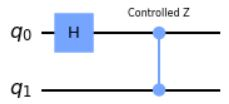
\includegraphics[scale=0.8]{cz-gate}\]
    \item (5 points) Can the controlled Z gate matrix be written as the tensor product of two matrices? Prove or disprove.
    \item (15 points) Consider standard quantum teleportation. Imagine Alice has the incredible power to transmit exactly one bit to Bob instantaneously (faster than the speed of light whoa). Let's think about how this changes Bob's situation.
    \begin{enumerate}
        \item What is the probability that Bob obtains the correct state?
        \item What does Bob know about his state if Alice tells him the first qubit's value of her system?
        \item What does Bob know about his state if Alice tells him the second qubit's value of her system?
        \item If Bob only cares about getting the probabilities of his basis states right and doesn't care about the phase of his system, which qubit would he want Alice to send?
    \end{enumerate}
    \item (5 points) Explain why using just a single EPR pair, Bob cannot obtain Alice's state any more than 50\% of the time without communication and ignoring phase differences.
    \item (10 points) Consider the entangled state: 
    \[\ket{\psi} = \frac{1}{\sqrt{2}}(\ket{00}+\ket{11})\]
    Show that applying a general U gate to the first qubit still results in an entangled state.
    \item (10 points) Recreate the table on slide 9 in Lecture 10 (i.e. what action Bob should take for each measurement Alice could observe) if Alice and Bob used the below EPR pair to accomplish quantum teleporation.
    \[\ket{\psi} = \frac{1}{\sqrt{2}}(\ket{01}-\ket{10})\]
    \item (5 points) Suppose you have the following state:
    \begin{multline} \ket{\psi} = 
        \alpha_0\ket{000} + \alpha_1\ket{001} +
                    \alpha_2\ket{010} + \alpha_3\ket{011}  \\
                    + \alpha_4\ket{100} + \alpha_5\ket{101} +
                    \alpha_6\ket{110} + \alpha_7\ket{111}
    \end{multline}
    Furthermore, suppose $|\alpha_0|^2 = 0.5$, $|\alpha_1|^2 = 0.25$, and $|\alpha_5|^2 = 0.125$. Suppose you measure the first two qubits and see $00$. What is the probability of measuring 0 on the third qubit?
    \item (Bonus, up to 3 points) Write one interesting question related to the content of this homework, and indicate the correct answer. The question can be multiple-choice or free-response.  Interesting questions get credit here;  sufficiently good questions might appear on an exam.
\end{enumerate}



\end{document}